\documentclass{../../../fal_assignment}
\graphicspath{ {../../../} }

\usepackage{amsmath}
\usepackage{enumitem}
\setlist{nosep} % Make enumerate / itemize lists more closely spaced
\usepackage[T1]{fontenc} % http://tex.stackexchange.com/a/17858
\usepackage{url}
\usepackage{todonotes}
\usepackage{graphicx}
\usepackage{subcaption}
\usepackage{hyperref}

\hypersetup{
	colorlinks=true, 
   	urlcolor=black,
	linkcolor=black
}

\usepackage{listings}
\lstset{
	basicstyle=\ttfamily,
	frame=single,
	showstringspaces=false,
	breaklines=false,
	prebreak={\space\hbox{\textcolor{gray}{$\hookleftarrow$}}}
}
\lstset{
	commentstyle=\ttfamily\textit,
	keywordstyle=\ttfamily\textbf,
	stringstyle=\ttfamily,
	rulecolor=\color{black}
}
\lstset{language=C++}

\newcommand{\colvec}[2]{\begin{pmatrix}#1\\#2\end{pmatrix}}
\newcommand{\colxy}[1]{\colvec{x_{#1}}{y_{#1}}}

\setenumerate[0]{label=(\alph*)}

\title{Worksheet D}
\author{Kate Bergel}
\module{COMP270}
\version{1.0}

\begin{document}

\maketitle

\section*{Introduction}

In this worksheet you will make use of the profiling tools in Visual Studio\footnote{Or similar tool of your choice.} to analyse the performance of a simple game, using the results to guide your efforts to improve efficiency.

Begin by \textbf{forking} the following git repository:

\begin{center}
	\url{https://github.com/Falmouth-Games-Academy/comp270-worksheet-D}
\end{center}

\textbf{Complete} the tasks described below, remembering to \textbf{commit} your work regularly.
To submit your work, open a \textbf{pull request} from your forked repository to the original repository.

\textbf{Notes}:
\begin{itemize}
	\item Completing the worksheet requires writing answers to the questions posed, as well as implementing code changes. The written answers should be fairly short, so can be included in the comments, git commit messages, or readme file.
	\item Profiling results should also be included to show the effect of your code changes. If you can export the data as a text file, it may be included in this format; otherwise, write down the key information in your answers/comments.
	\item Some of the implementations in the tasks below may be concentrated on a particular function or data structure, however you are free to modify any parts of the code you think appropriate. Make sure to justify your changes in code comments and/or git commit messages.
	\item Tasks 2 and 3 can be implemented in any order, and task 4 may be attempted without their being completed, but task 1 \textit{must} be completed first.
\end{itemize}

\section*{Background}

\begin{figure}[ht]
	\begin{center}
		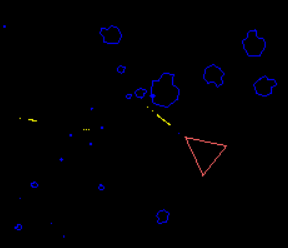
\includegraphics[width=0.5\linewidth]{asteroids}
	\end{center}
	\caption{The game in action}
	\label{fig:game}
\end{figure}

The code provided implements the basic features of an asteroids game: manoeuvring a “spaceship” around the screen and firing bullets at space rocks to break them into smaller fragments, as shown in Figure~\ref{fig:game}. Features such as scoring and health/player lives are not implemented as these are not necessary for (and would possibly interfere with) the main focus of the tasks below - which is to make sure that the game will continue to play smoothly and with the best frame-rate possible, even with large numbers of objects.

The game uses the following keyboard controls:
\begin{itemize}
	\item \lstinline{up arrow}: applies a thrust in the direction the spaceship is facing
	\item \lstinline{right/left arrow}: rotates the spaceship clockwise/anticlockwise
	\item \lstinline{space bar}: fires a bullet from the front of the spaceship
\end{itemize}

\section*{Task 1: making your benchmark}

\begin{enumerate}
	\item The main bulk of the code runs in \lstinline{Application::update()}, which handles the game logic, and \lstinline{Application::render()}, which deals with the drawing. \textbf{Read} through these functions, and the ones they call (directly or indirectly), looking for obvious inefficiencies.\\
\textbf{List} any that you spot, and \textbf{state} how they might cause problems. Where do you think most of the work will be done?\\
	\item Now build the code and play through the game for a few minutes, shooting as many asteroids as you can. \textbf{Write down} any observations about the performance or other issues, and potential causes; these form hypotheses to test using profiling.\\
	\item In order for benchmarks to be useful, they should be run on a reproducible test case. Since user input is likely to vary between runs, \textbf{modify} some of the values\footnote{Hint: the asteroid spawning settings are in \lstinline{Application.h}.} and add logic to create a scenario that will push the code by generating a reasonably large number of objects, with minimal input from the player\footnote{Ideally none.}. Make sure that your test case will be representative, and call all the game code\footnote{Including, for example, breaking the asteroids into pieces.}.\\
\textbf{Commit} your changes, so that you can use this test case in the remaining tasks.\footnote{Normally, you should make sure to remove any such 'hacks' before committing your final solution, but don't worry about that for this assignment.}\\
	\item Run the Visual Studio CPU profiler (or other tool of your choice) to measure the times taken by the various functions. \textbf{Examine} the results and \textbf{state} which functions\footnote{Of the ones in the actual game code only - ignore SDL and any other 3rd party or Windows native code.} are using the largest percentage of time. Are they the ones you predicted? If not, \textbf{explain} what might be causing the results.\\
	\item Now run the memory profiler, remembering to take snapshots at the start and regular intervals. Do these results match your expectations? \textbf{Explain} why (or why not).
\end{enumerate}

\section*{Task 2: insider knowledge}

In order to make the asteroids explode at an appropriate time, the code has to check whether any bullets are inside each asteroid's boundary. This kind of collision detection is often one of the most computationally intensive parts of a game.

The algorithm implemented in \lstinline{Asteroid::pointIsInside()} is known as the "angle summation test", but there are several alternative approaches to testing whether a point is inside a polygon, as described here: \url{https://erich.realtimerendering.com/ptinpoly/}

\begin{enumerate}
	\item See if you can increase the efficiency of \lstinline{Asteroid::pointIsInside()} by \textbf{implementing} an alternative algorithm. \textbf{State} which one you have chosen and justify your choice in the comments.\\
\textbf{Re-run} the CPU profiler on your test case and \textbf{state} how much the time has improved.\\
	\item Can you improve the average efficiency of this function even further by reducing the number of times the full point-in-polygon test is carried out?\\
\textbf{Implement} an "early exit" condition to avoid testing bullets that are "obviously" far away from the asteroid, then \textbf{re-run} the CPU profiler again to see if it has helped.
\end{enumerate}

\section*{Task 3: space debris}

Both the asteroids and bullets are stored in \lstinline{std::vector} containers, with new objects being added using \lstinline{push_back()} whenever the space bar is pressed, an asteroid is shattered or a new one is spawned in \lstinline{Application::update()}.

\begin{enumerate}
	\item Thinking about the CPU and memory profiling results from Task 1, \textbf{list} the pros and cons of the current implementation using \lstinline{std::vector}.\\
	\item Use the debugger, or a manual counting mechanism, to keep track of how many objects are in the scene. \textbf{Compare} this number to what you can see on the screen - do the figures correspond? \textbf{Explain} why this is and how it might be affecting the performance.\\
	\item \textbf{Describe} two or more different ways you could compensate for and/or reasonably limit the large number of objects that are being generated, without affecting the game experience\footnote{Ideally keeping the asteroids spawning at a consistent rate for the duration.}.\\
Might using a different data structure be more appropriate? Which one, and/or why (not)?\\
	\item \textbf{Implement} (at least) one of your ideas above, testing the effects on performance as usual.
\end{enumerate}

\section*{Task 4: how low can you go?}

\begin{enumerate}
	\item \textbf{Examine} your latest benchmarks (re-running them if necessary) to see which other operations are taking up a significant proportion of the time\footnote{You may get more information by profiling in debug mode.}. \textbf{List} which of these you think it might be possible to improve upon.\\
	\item \textbf{Implement} at least two changes to address one or more inefficiencies, \textbf{explaining} your motivations in the comments/commit messages and noting the results of profiling after each one.\\
	\item \textbf{Describe} any further enhancements you think might be beneficial to the game's performance.
\end{enumerate}

\begin{markingrubric}
	\firstcriterion{Basic competency threshold}{30\%}
		\grade\fail	A reasonable attempt at the worksheet was not submitted by the formative deadline.
	\gradespan{5}{A reasonable attempt at the worksheet was submitted by the formative deadline.
		\par		There is no evidence of academic misconduct.}
		
    \criterion{Functional coherence}{40\%}
        \grade\fail None of the tasks have been attempted.
		\grade Task 1 has been attempted and partially completed.
		\grade Task 1 has been successfully completed.
		\grade Two tasks (including task 1) have been successfully completed.
		\grade Three tasks (including task 1) have been successfully completed.
		\grade All four tasks have been successfully completed.

    \criterion{Maintainability}{30\%}
        \grade \fail The code is only sporadically commented, if at all, or comments are unclear.
            \par Few identifier names are clear or inappropriate.
            \par Code formatting hinders readability.
        \grade The code is well commented.
            \par Some identifier names are descriptive and appropriate.
            \par An attempt has been made to adhere to a consistent formatting style.
             \par There is little obvious duplication of code or of literal values.           
        \grade The code is reasonably well commented.
            \par Most identifier names are descriptive and appropriate.
            \par Most code adheres to a sensible formatting style.
             \par There is almost no obvious duplication of code or of literal values.   
        \grade The code is reasonably well commented, with appropriate high-level documentation.
            \par Almost all identifier names are descriptive and appropriate.
            \par Almost all code adheres to a sensible formatting style.
             \par There is no obvious duplication of code or of literal values. Some literal values can be easily ``tinkered''. 
        \grade The code is very well commented, with comprehensive appropriate high-level documentation.
            \par All identifier names are descriptive and appropriate.
            \par All code adheres to a sensible formatting style.
             \par There is no obvious duplication of code or of literal values. Most literal values are, where appropriate, easily ``tinkered''.  
        \grade The code is commented extremely well, with comprehensive appropriate high-level documentation.
            \par All identifier names are descriptive and appropriate.
            \par All code adheres to a sensible formatting style.
            \par There is no duplication of code or of literal values. Nearly all literal values are, where appropriate, easily ``tinkered''.  
\end{markingrubric}

\end{document}
